\documentclass[conference]{IEEEtran}
\IEEEoverridecommandlockouts
% The preceding line is only needed to identify funding in the first footnote. If that is unneeded, please comment it out.
\usepackage{cite}
\usepackage{amsmath,amssymb,amsfonts}
\usepackage{algorithmic}
\usepackage{graphicx}
\usepackage{textcomp}
\usepackage{xcolor}
\usepackage{hyperref}
\hypersetup{
    citecolor=blue,
    colorlinks=true,      
    urlcolor=blue,
}
\def\BibTeX{{\rm B\kern-.05em{\sc i\kern-.025em b}\kern-.08em
    T\kern-.1667em\lower.7ex\hbox{E}\kern-.125emX}}
\begin{document}

\title{Flappy Bird AI based on Neuroevolution of Augmenting Topologies}

\author{\IEEEauthorblockN{1\textsuperscript{st} M. Osama Asif}
\IEEEauthorblockA{\textit{BS-CS 17L-4295} \\
\textit{FAST-NU}\\
Lhr, Pak}
\and
\IEEEauthorblockN{2\textsuperscript{nd} M. Ibraheem Waheed}
\IEEEauthorblockA{\textit{BS-CS 17L-4315} \\
\textit{FAST-NU}\\
Lhr, Pak}
\and
\IEEEauthorblockN{3\textsuperscript{rd} Waleed Iqbal}
\IEEEauthorblockA{\textit{BS-CS 17L-4032} \\
\textit{FAST-NU}\\
Lhr, Pak}
\and
\IEEEauthorblockN{4\textsuperscript{th} M. Husnain Maqsood}
\IEEEauthorblockA{\textit{BS-CS 17L-4228} \\
\textit{FAST-NU}\\
Lhr, Pak}
}

\maketitle

\begin{abstract}
This report deals with the project we conducted as part of our AI course at FAST-NU. The project deals with the creation of an Artificial Intelligence using Neuroevolution of Augmenting Topologies (NEAT) that can play the famous Flappy Bird game perfectly after minimal amount of generations/learning. NEAT is a way of evolving neural networks using genetic algorithm. We used an already available implementation of Flappy Birds and used that to build our NEAT AI upon. For the purpose of implementing NEAT we used NEAT-Python library, which provides us with an easy to use abstraction of already implemented basic functionality. The Results are very promising; using tanh function, we are able to make an AI that easily learns to play amazingly within 2, or 3 generations on average (with a 50 population size per generation).
\end{abstract}

\begin{IEEEkeywords}
AI, NEAT, Genetic Algorithms, Neural Networks, tanh, Flappy Birds, Python
\end{IEEEkeywords}

\section{Introduction}
In our Artificial Intelligence course at FAST-NU, we wrote a simple AI using Neuroevolution of Augmenting Topologies (NEAT) that is able to play the famous Flappy Bird game far better than a human being can. The language we used for our project is Python, since as opposed to other low level languages it provides a far better abstraction that allows us to easily implement an AI. The Flappy Bird code we used is an already implemented one by someone else found on github. For the purpose of NEAT we used NEAT-Python library, which gives us an easy to use abstraction of the basic NEAT implementation.

\section{Neuroevolution of Augmenting Topologies (NEAT)}

\subsection{Encoding}
NEAT, like any other genetic algorithm is heavily influenced by natural processes of evolution. Similar to nature, they have a genotype and a phenotype. Genotype is the representation of the data that makes up the gene (basic unit), and phenotype is the actual visualization of the that genotype. How to encode the data becomes the main question, because it heavily influences how the further processes will be conducted. This includes mutation, selection etc.

Encoding can be of two types, direct and indirect. \textbf{Direct Encoding} will explicitly specify everything about an individual. If it represents a neural network this means that each gene will directly be linked to some node, connection, or property of the network (can be binary, or graph encoding i.e. various node connections etc). So a direct connection between genotype and phenotype exists. On the other hand \textbf{Indirect Encoding} uses parameters and inputs to define how a unit will be represented. This method although compact, poses the problem that a massive amount of knowledge is required for the underlying usage of individual (unit) since only than can we define an unbiased parameters etc.

NEAT uses direct encoding for above mentioned reasons. It uses two lists of genes, a series of nodes and connections (Fig.~\ref{fig1}). Input and output nodes are not evolved, and hidden can be added or removed. Connections specify which node is connected and how, along with weight for the connection, wether it's enabled and innovation number (explain under Mutation).

\begin{figure}[htbp]
\centering{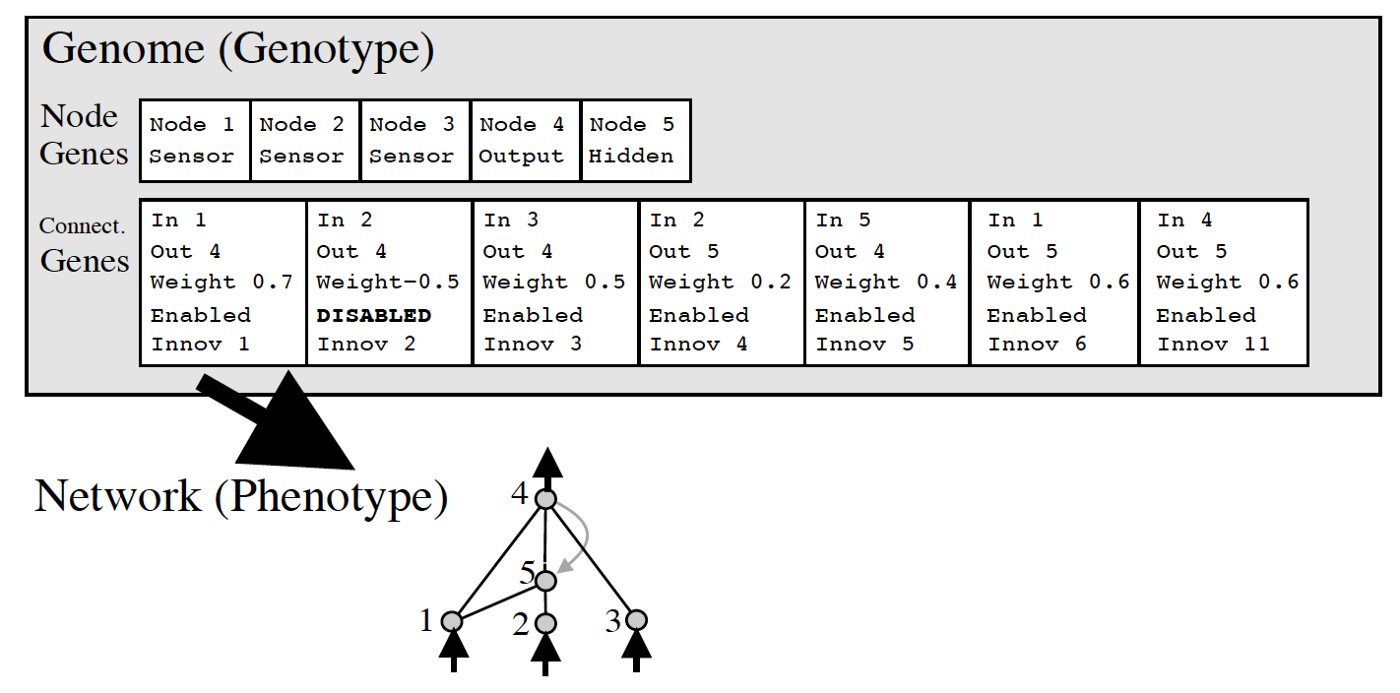
\includegraphics[scale=0.2]{fig1.png}}
\caption{Encoding scheme for NEAT}
\label{fig1}
\end{figure}

\subsection{Mutation}

Mutation can be done either by changing existing connections between nodes, or by adding new connections. New connections are always added between nodes that already contain connections. The old connection is disabled(but still exists in genome). The connection from starting node (in node) is given the same weight as old connection, but the connection from end node is given a weight of 1 (found to be able to resolve issues according to original paper) \cite{b2}. There is one exception to this method; when a connection is added between root and end node, they are assigned random weights. 

\begin{figure}[htbp]
\centering{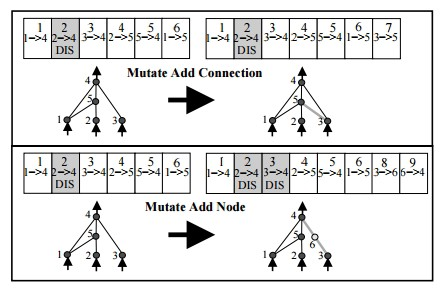
\includegraphics[scale=0.5]{fig2.jpg}}
\caption{Mutation visualization}
\label{fig2}
\end{figure}

\subsection{Competing Conventions}

This is taken from the original paper \cite{b2}. The idea is that randomly mutating neural networks can result in networks that are inefficient and useless. One issue can be that both networks being mutated are dependent on a central node, that get recombined from both sides, it will cause an issue. Another issue is different sized genomes, how to crossover them? This is handled in nature by homology, matching/aligning genomes based on similar traits. NEAT uses historical markings (Fig.~\ref{fig3}). New evolutions marked with historical numbers, so that less chance of useless crossover. Marking assigned each time gene, or connection is formed (Fig.~\ref{fig4}). 

\begin{figure}[htbp]
\centering{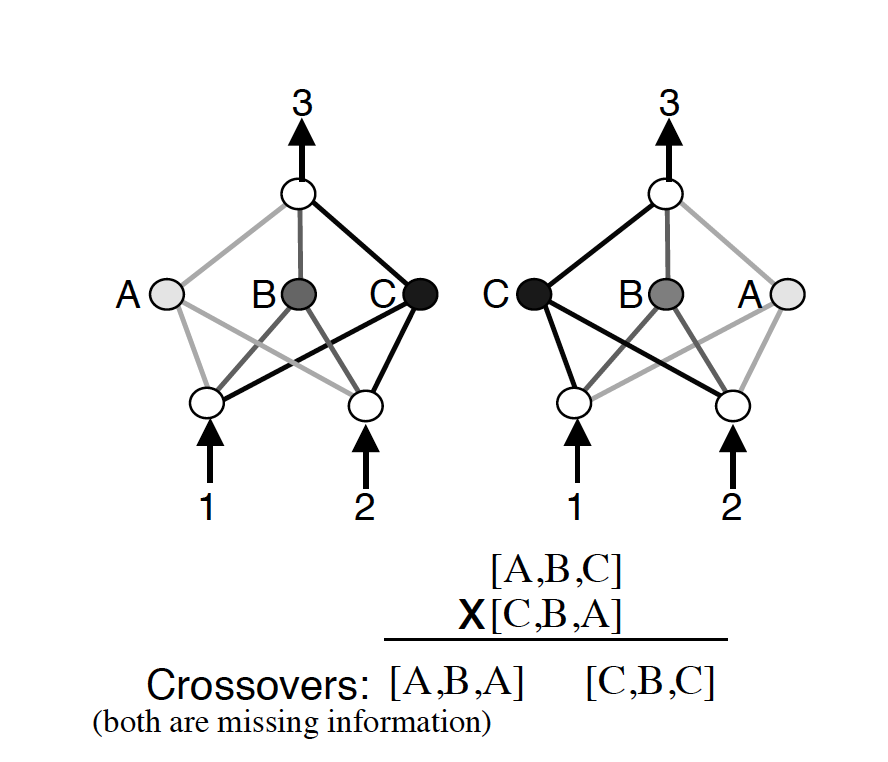
\includegraphics[scale=0.3]{fig3.png}}
\caption{Missing information/incompatibility}
\label{fig3}
\end{figure}

\begin{figure}[htbp]
\centering{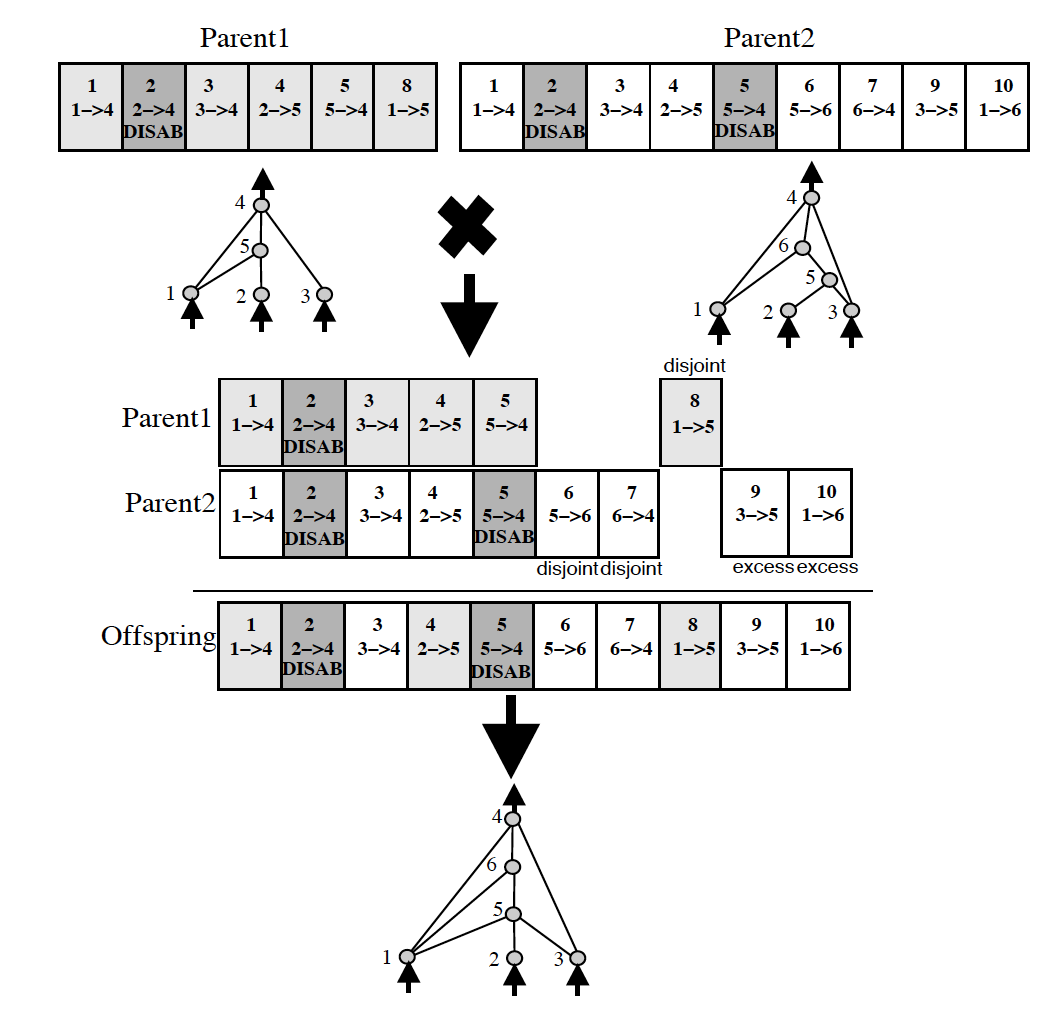
\includegraphics[scale=0.2]{fig4.png}}
\caption{Usage of historical markings}
\label{fig4}
\end{figure}

\subsection{Speciation}

In NEAT it was suggested that most new evolutions are not good ones. In fact, adding a new connection or node before any optimization of weights have occurred often leads to a lower performing individual. This puts new structures at a disadvantage. Speciation is technique of protecting new structures so they can optimize before getting removed.

Population divided into multiple species based on connections etc. Competition only occurs within species, so that new individuals are explored before they die.

More than that, NEAT takes things one step forward through something called explicit fitness sharing. That means that individuals share how well they are doing across the species, boosting up higher performing species, though still allowing for other species to explore their structure optimization before being out evolved. \cite{b2}

\subsection{Minimal Structure}

NEAT never begins with a highly advanced NN. Every network in the beginning is only made up of input and output nodes, there are no hidden nodes/layers. Overtime it evolves the network into highly specialized and complex networks, only if they are useful. This idea along with speciation mentioned above serves the purpose perfectly. \cite{b2}

So all in all NEAT is a very good technique of developing Neural Networks overtime, as much as needed, to come with the best option to use to solve the problem at hand.

\section{NEAT-Python}

NEAT-Python is a Python based implementation of of Neuroevolution of Augmenting Topologies. It is very well written and abstracted implementation, that allows the user to provide minimal input in order for it to work as intended. The main input is a configuration file, that contains population size, node connection information, activation function to use, and the function to choose the best genome to name a few. Along with this, the we need to provide it with a evaluation function and count of generations, and it takes care of everything else for us. So, for the purpose of our project we used this library in order to implement the NEAT based AI. \cite{b3}

\section{Flappy Bird}

Flappy Bird (Fig.~\ref{fig5}) is a mobile game that came out back in 2013, made by a Vietnamese artist and developer, and was played by millions of people around the world. It became famous because of it's simple, yet difficult mechanism that requires alot of attention by the player. The game is essentially a 2D side scroller where pipes (vertically in line with each other) move from the right towards the bird (player) on the left. The pipes have varying lengths (randomly generated) and there is an opening between them that the bird needs to pass inorder to keep on going. A soon as it hits a pipe or ground, it dies. The control is simply to press space bar inorder to make the bird jump, not pressing it makes the bird fall, and the player needs to find the balance between this.

The game we have used in our project has been taken from github. The game suited us because it was written with minimal code, and worked perfectly. We implemented our NEAT AI on top of it, and also added some aesthetic features to the game itself.

\begin{figure}[htbp]
\centering{
\includegraphics[scale=1.2]{fig5.jpg}}
\caption{Game Screen of Flappy Birds}
\label{fig5}
\end{figure}

\section{Implementation}

\subsection{NEAT-Python Configurations}

The template file for NEAT configuration was taken from the actual NEAT-Python documentation and the required fields were tweaked \cite{b3}. The file looks something like in (Fig.~\ref{fig6}). We found that most of the configurations worked perfectly for our case. However there were still a few values that we had to change to find the best working AI. fitness\_criterion was changed to max, which defines the function used to pick the best genome of a generation. pop\_size was also changed. We found through (given in next section) that anything above or equal to 50 was enough for good results. Activation function was also changed to tanh, since we found for the evaluation function, the output of \-1 to 1 gave promising results.

\begin{figure}[htbp]
\centering{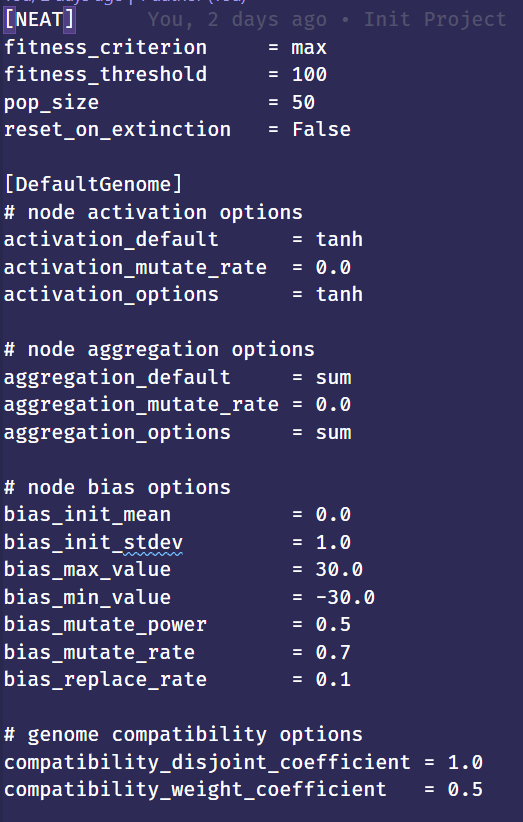
\includegraphics[scale=0.7]{fig6.png}}
\caption{Configuration File for NEAT}
\label{fig6}
\end{figure}

\subsection{Evaluation Function}

The evaluation function for this game was kept quite simple. There are three main conditions that make it work. The first condition is to detect collision between the bird and any of the two pipes that are closest to it on the screen. Then if if it hits any pipe out of those two, the fitness score is decreased by 1 and the bird removed. Ground collision is not given a penalty, that was found to be unnecessary. 0.1 is added to fitness of the bird per frame. Finally 5 is added to it each time it passes through a pipe successfully.

\section{Results}

The Result we conducted used 6 different population sizes with 3 different score goal to achieve. The population sizes used were, 10, 20, 30, 40, 50 and 60. Whereas the score goal values were 100, 200 and 300. During this everything else was kept the same and max generations allowed everytime was 50. The line graph (Fig.~\ref{fig7}) summarizes our results.

\begin{figure}[htbp]
\centering{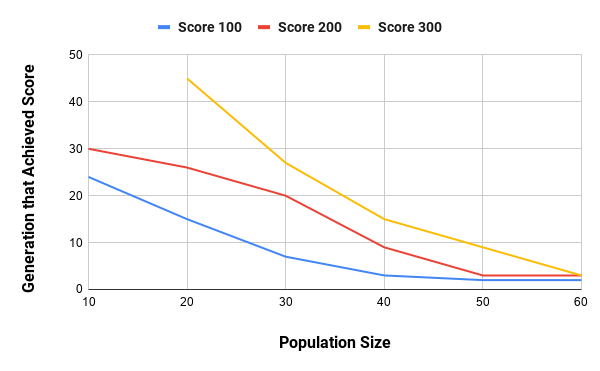
\includegraphics[scale=0.3]{fig7.png}}
\caption{"Generation that achieved score vs Population size" graph}
\label{fig7}
\end{figure}

\section{Conclusion}

So in retrospect, the use of NEAT-Python with population size of 50, and tanh activation function has provided with a very efficient AI that is able to learn the game within 2-3 generations, and go onto get very good scores.

\begin{thebibliography}{00}
\bibitem{b1} Hunter Heidenreich, "NEAT:An Awesome Approach to NeuroEvolution", towardsdatasciene.com, Jan. 4, 2019. [Online]. Available: \url{https://towardsdatascience.com/neat-an-awesome-approach-to-neuroevolution-3eca5cc7930f}. [Accessed June 12, 2020]
\bibitem{b2} K. O. Stanley, R. Miikkulainen, "Evolving Neural Networks through Augmenting Topologies", Department of Computer Science, University of Texas, 2002. Available: \url{http://nn.cs.utexas.edu/downloads/papers/stanley.ec02.pdf}. [Accessed June 12, 2020]
\bibitem{b3} NEAT-Python, "NEAT-Python Documentation". [Online]. Available: \url{https://neat-python.readthedocs.io/en/latest/}. [Accessed June 12, 2020]
\bibitem{b4} Murat Vurucu, "How to we teach a machine to program itself? NEAT learning", towardsdatasciene.com, July 25, 2017. [Online]. Available: \url{https://towardsdatascience.com/how-do-we-teach-a-machine-to-program-itself-neat-learning-bb40c53a8aa6}. [Accessed June 12, 2020]
\bibitem{b5} Hunter Heidenreich, "HyperNEAT: Powerful, Indirect Neural Network Evolution", towardsdatasciene.com, Jan. 10, 2019. [Online]. Available: \url{https://towardsdatascience.com/hyperneat-powerful-indirect-neural-network-evolution-fba5c7c43b7b}. [Accessed June 12, 2020]
\bibitem{b6} Wikipedia, "NeuroEvolution of Augmenting Topologies", wikipedia.com, Apr. 16, 2020. [Online]. Available: \url{https://en.wikipedia.org/wiki/Neuroevolution_of_augmenting_topologies}. [Accessed June 12, 2020]
\end{thebibliography}

\end{document}
